\documentclass[12pt]{beamer}
\usepackage{../Estilos/BeamerFC}
\usepackage{../Estilos/ColoresLatex}
\usepackage{enumitem}
% \usefonttheme{serif}
\usetheme{Copenhagen}
\usecolortheme{wolverine}
%\useoutertheme{default}
\setbeamercovered{invisible}
% or whatever (possibly just delete it)
\setbeamertemplate{section in toc}[sections numbered]
\setbeamertemplate{subsection in toc}[subsections numbered]
\setbeamertemplate{subsection in toc}{\leavevmode\leftskip=3.2em\rlap{\hskip-2em\inserttocsectionnumber.\inserttocsubsectionnumber}\inserttocsubsection\par}
% \setbeamercolor{section in toc}{fg=blue}
% \setbeamercolor{subsection in toc}{fg=blue}
% \setbeamercolor{frametitle}{fg=blue}
\setbeamertemplate{caption}[numbered]

\setbeamertemplate{footline}
\beamertemplatenavigationsymbolsempty
\setbeamertemplate{headline}{}


\makeatletter
% \setbeamercolor{section in foot}{bg=gray!30, fg=black!90!orange}
% \setbeamercolor{subsection in foot}{bg=blue!30}
% \setbeamercolor{date in foot}{bg=black}
\setbeamertemplate{footline}
{
  \leavevmode%
  \hbox{%
  \begin{beamercolorbox}[wd=.333333\paperwidth,ht=2.25ex,dp=1ex,center]{section in foot}%
    \usebeamerfont{section in foot} \insertsection
  \end{beamercolorbox}%
  \begin{beamercolorbox}[wd=.333333\paperwidth,ht=2.25ex,dp=1ex,center]{subsection in foot}%
    \usebeamerfont{subsection in foot}  \insertsubsection
  \end{beamercolorbox}%
  \begin{beamercolorbox}[wd=.333333\paperwidth,ht=2.25ex,dp=1ex,right]{date in head/foot}%
    \usebeamerfont{date in head/foot} \insertshortdate{} \hspace*{2em}
    \insertframenumber{} / \inserttotalframenumber \hspace*{2ex} 
  \end{beamercolorbox}}%
  \vskip0pt%
}
\makeatother

\makeatletter
\patchcmd{\beamer@sectionintoc}{\vskip1.5em}{\vskip0.8em}{}{}
\makeatother

% %\newlength{\depthofsumsign}
% \setlength{\depthofsumsign}{\depthof{$\sum$}}
% \newcommand{\nsum}[1][1.4]{% only for \displaystyle
%     \mathop{%
%         \raisebox
%             {-#1\depthofsumsign+1\depthofsumsign}
%             {\scalebox
%                 {#1}
%                 {$\displaystyle\sum$}%
%             }
%     }
% }
% \def\scaleint#1{\vcenter{\hbox{\scaleto[3ex]{\displaystyle\int}{#1}}}}
% \def\scaleoint#1{\vcenter{\hbox{\scaleto[3ex]{\displaystyle\oint}{#1}}}}
% \def\bs{\mkern-12mu}


\title{Leyes de Newton}
\subtitle{Tema 1 - Dinámica de una partícula}
% \date{}
% \author{M. en C. Gustavo Contreras Mayén.}


\newcommand\RBox[1]{%
  \tikz\node[draw,rounded corners,align=center,] {#1};%
}

\AtBeginDocument{\RenewCommandCopy\qty\SI}
\ExplSyntaxOn
\msg_redirect_name:nnn { siunitx } { physics-pkg } { none }
\ExplSyntaxOff

\resetcounteronoverlays{saveenumi}

\begin{document}
\fontsize{14}{14}\selectfont
\spanishdecimal{.}
\maketitle

\section*{Contenido}
\frame[allowframebreaks]{\frametitle{Contenido} \tableofcontents[currentsection, hideallsubsections]}

\section{Leyes de Newton}
\frame[allowframebreaks]{\frametitle{Temas a revisar} \tableofcontents[currentsection, hideothersubsections]}
\subsection{Primera revisión}

\begin{frame}
\frametitle{Objetivo de la mecánica}
La mecánica es una rama de la física que se ocupa del estudio del movimiento de los cuerpos y las fuerzas que actúan sobre ellos.
\end{frame}
\begin{frame}
\frametitle{Objetivo de la mecánica}
Su objetivo principal es describir, analizar y predecir el comportamiento de los sistemas físicos en función de leyes matemáticas.
\end{frame}
\begin{frame}
\frametitle{Objetivo de la mecánica}
Como herramientas matemáticas se considerarán entre otros:
\setbeamercolor{item projected}{bg=coquelicot,fg=white}
\setbeamertemplate{enumerate items}{%
\usebeamercolor[bg]{item projected}%
\raisebox{1.5pt}{\colorbox{bg}{\color{fg}\footnotesize\insertenumlabel}}%
}
\begin{enumerate}
\item Ecuaciones diferenciales.
\item Matrices.
\item Cálculo vectorial.
\item Álgebra compleja.
\end{enumerate}
\end{frame}
\begin{frame}
\frametitle{Objetivo de la mecánica}
Estas leyes permiten entender fenómenos físicos que ocurren en nuestra vida diaria y en escalas macroscópicas.
\end{frame}
\begin{frame}
\frametitle{Alcance de la mecánica clásica}
La mecánica clásica no es adecuada para estudiar fenómenos que ocurren a velocidades cercanas a la velocidad de la luz (\textocolor{red}{relatividad}) \pause o a escala subatómica (\textocolor{ao}{mecánica cuántica}).
\end{frame}

% Ref. Fowles (2004) - 2.1

\subsection{Leyes de Newton}

% \begin{frame}
% \frametitle{Partícula puntual}
% Una \textocolor{cobalt}{partícula puntual}, que también se le conoce como masa puntual, punto material, o de manera más clara: \textocolor{carmine}{partícula}.
% \end{frame}
% \begin{frame}
% \frametitle{Partícula puntual}
% Es una idealización de un objeto cuando solo nos interesa el estudio de la posición de un punto de ese objeto, haciendo a un lado propiedades del mismo: extensión, color, volumen, etc.
% \end{frame}

\begin{frame}
\frametitle{Las leyes de Newton}
En sus Principia de 1687, Isaac Newton estableció sus propias leyes fundamentales del movimiento, que cambiarían para siempre la percepción del mundo por parte de la humanidad:
\end{frame}
\begin{frame}
\frametitle{Primera ley}
\setbeamercolor{item projected}{bg=cobalt,fg=white}
\setbeamertemplate{enumerate items}{%
\usebeamercolor[bg]{item projected}%
\raisebox{1.5pt}{\colorbox{bg}{\color{fg}\footnotesize\insertenumlabel}}%
}
\begin{enumerate}[label=\Roman*.]
\item Todo cuerpo continúa en su estado de reposo o de movimiento uniforme en línea recta, a menos que se vea obligado a cambiar ese estado por fuerzas que se le imponen.
\seti
\end{enumerate}
\end{frame}
\begin{frame}
\frametitle{Segunda ley}
\setbeamercolor{item projected}{bg=cobalt,fg=white}
\setbeamertemplate{enumerate items}{%
\usebeamercolor[bg]{item projected}%
\raisebox{1.5pt}{\colorbox{bg}{\color{fg}\footnotesize\insertenumlabel}}%
}
\begin{enumerate}[label=\Roman*.]
\conti
\item El cambio de movimiento es proporcional a la fuerza motriz impuesta y se produce en la dirección de la línea en la que se impone esa fuerza.
\seti
\end{enumerate}
\end{frame}
\begin{frame}
\frametitle{Tercera ley}
\setbeamercolor{item projected}{bg=cobalt,fg=white}
\setbeamertemplate{enumerate items}{%
\usebeamercolor[bg]{item projected}%
\raisebox{1.5pt}{\colorbox{bg}{\color{fg}\footnotesize\insertenumlabel}}%
}
\begin{enumerate}[label=\Roman*.]
\conti
\item A cada acción se le impone siempre una reacción igual; o bien, las acciones mutuas de dos cuerpos entre sí son siempre iguales y están dirigidas a partes contrarias.
\end{enumerate}
\end{frame}
\begin{frame}
\frametitle{Interpretación de las leyes}
Las leyes de Newton sobre el movimiento pueden considerarse como una receta para calcular o predecir el movimiento posterior de una partícula (o sistema de partículas), dado el conocimiento de su \textocolor{cobalt}{posición} y \textocolor{byzantium}{velocidad} en un instante determinado.
\end{frame}
\begin{frame}
\frametitle{Interpretación de las leyes}
Estas leyes, por sí mismas, no dicen nada sobre la razón por la que un sistema físico determinado se comporta como lo hace.
\end{frame}
\begin{frame}
\frametitle{Interpretación de las leyes}
Newton fue bastante explícito sobre esa deficiencia.
\\
\bigskip
\pause
Se negó a especular (al menos en forma impresa) sobre por qué los objetos se mueven como lo hacen.
\end{frame}
\begin{frame}
\frametitle{Interpretación de las leyes}
Cualquier \enquote{mecanismo} que se escondiera detrás del funcionamiento de los sistemas físicos permaneció oculto para siempre a los ojos de Newton.
\end{frame}
\begin{frame}
\frametitle{Interpretación de las leyes}
Simplemente afirmó que, por la razón que sea, \textocolor{debianred}{así es como funcionan las cosas}, \pause como lo demuestra el poder de su receta de cálculo para predecir con asombrosa precisión, la evolución de los sistemas físicos puestos en movimiento.
\end{frame}
\begin{frame}
\frametitle{Interpretación de las leyes}
Mucho se ha aprendido desde la época de Newton, pero un hecho básico la ley física persiste: \pause \emph{las leyes del movimiento son prescripciones matemáticas que nos permiten predecir con precisión el movimiento futuro de los sistemas físicos}, dado el conocimiento de su estado actual.
\end{frame}
\begin{frame}
\frametitle{Interpretación de las leyes}
Las leyes describen cómo funcionan las cosas.
\\
\bigskip
\pause
No nos dicen por qué.
\end{frame}

\subsection{Primera ley}

\begin{frame}
\frametitle{La inercia}
La primera ley describe una propiedad común de la materia, \pause a saber, \textocolor{amethyst}{la inercia}.
\end{frame}
\begin{frame}
\frametitle{La inercia}
En términos generales, la inercia es la resistencia de una materia a que se modifique su movimiento.
\end{frame}
\begin{frame}
\frametitle{La inercia}
Si una partícula está en reposo, se resiste a ser movida, \pause es decir, se requiere una fuerza para moverla.
\\
\bigskip
\pause
Si la partícula está en movimiento, se resiste a ser detenida. \pause Nuevamente, se requiere una fuerza para ponerla en reposo.
\end{frame}
\begin{frame}
\frametitle{La inercia}
%Casi parece como si la materia hubiera sido dotada de un aborrecimiento innato de la aceleración.
Sea como fuere, por la razón que sea, se necesita una fuerza para acelerar la materia.
\\
\bigskip
\pause
En ausencia de fuerzas aplicadas, la materia simplemente persiste en su estado de velocidad actual, para siempre.
\end{frame}
\begin{frame}
\frametitle{Sistema de referencia}
La descripción matemática del movimiento de una partícula requiere la selección de \textocolor{blue-violet}{un sistema (marco) de referencia}.
\end{frame}
\begin{frame}
\frametitle{Sistema de referencia}
Que es un conjunto de coordenadas en el espacio de configuración que se puede utilizar para especificar la posición, la velocidad y la aceleración de la partícula en cualquier instante de tiempo.
\end{frame}
\begin{frame}
\frametitle{Sistemas inerciales}
Un sistema de referencia en el que es válida la primera ley del movimiento de Newton se conoce como un \textocolor{cadmiumgreen}{sistema de referencia inercial}.
\end{frame}
\begin{frame}
\frametitle{Sistemas no inerciales}
Esta primera ley descarta los \textocolor{cerulean}{sistema de referencia acelerados como inerciales}, \pause porque un objeto que \enquote{realmente} se mueve a velocidad constante, en lugar de un sistema de referencia acelerado, parecería estar acelerado.
\end{frame}
\begin{frame}
\frametitle{Sistemas no inerciales}
Además, un objeto que se encuentra en reposo en dicho sistema se aceleraría con respecto al marco inercial. %Nuestra creencia en el concepto de inercia y la validez de las leyes del movimiento de Newton es tan fuerte que no podemos creer que la ley de Newton sea válida. verse obligado a inventar fuerzas "ficticias" para explicar la aparente falta de tolerancia de un objeto en un marco de referencia acelerado.
\end{frame}
\begin{frame}
\frametitle{Ejemplo de sistema no inercial}
Consideremos un observador dentro de un vagón de ferrocarril que se acelera por la vía con una aceleración $\vb{a}$.
\end{frame}
\begin{frame}
\frametitle{Ejemplo de sistema no inercial}
\begin{figure}
  \centering
  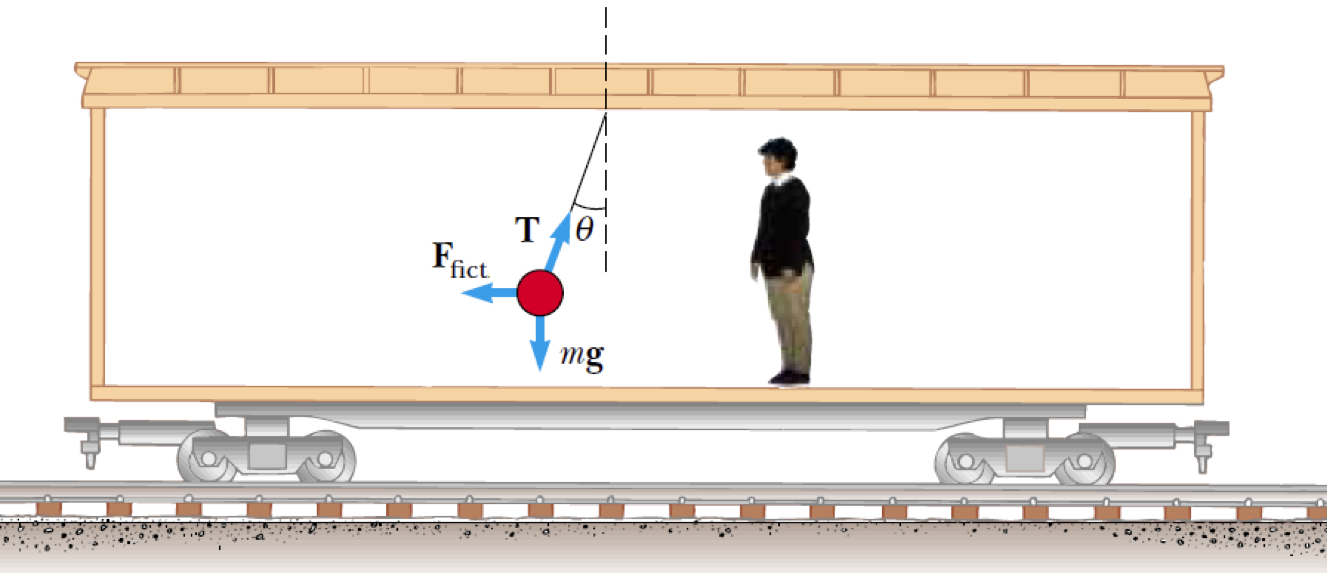
\includegraphics[scale=0.2]{Imagenes/Sistema_No_Inercial_01.png}
\end{figure}
\end{frame}
\begin{frame}
\frametitle{Ejemplo de sistema no inercial}
Supongamos que la plomada estuviera suspendida del techo del vagón.
\\
\bigskip
\pause
¿Cómo la vería el observador?
\end{frame}
\begin{frame}
\frametitle{Ejemplo de sistema no inercial}
El observador en el vagón está en un marco de referencia no inercial \pause y está en reposo con respecto a él.
\end{frame}
\begin{frame}
\frametitle{Ejemplo de sistema no inercial}
Él ve la plomada, también aparentemente en reposo, colgando en un ángulo $\theta$ con respecto a la vertical.
\end{frame}
\begin{frame}
\frametitle{Ejemplo de sistema no inercial}
Él sabe que, en ausencia de cualquier otra fuerza que no sea la gravedad y la tensión en la plomada, dicho dispositivo debería alinearse verticalmente.
\end{frame}
\begin{frame}
\frametitle{Ejemplo de sistema no inercial}
No es así, y concluye que alguna fuerza desconocida debe estar empujando o tirando de la plomada hacia la parte trasera del vagón.
\end{frame}
\begin{frame}
\frametitle{Ejemplo de sistema no inercial}
De hecho, él siente tal fuerza, como cualquiera que haya estado alguna vez en un vehículo acelerando sabe por experiencia propia.
\end{frame}
\begin{frame}
\frametitle{¿Cuándo un sistema es inercial?}
Una pregunta que surge naturalmente es: ¿cómo es posible determinar si un sistema de referencia dado constituye o no un marco inercial?
\\
\bigskip
\pause 
¡La respuesta no es trivial!
\end{frame}
\begin{frame}
\frametitle{¿Cuándo un sistema es inercial?}
Por ejemplo, si el vagón estuviera aislado del mundo exterior, \pause ¿cómo podría el observador saber que la fuerza aparente que hace que la plomada se desvíe de la vertical no se debe al hecho de que todo el vagón estuviera \enquote{desalineado} con la dirección de la gravedad?
\end{frame}
\begin{frame}
\frametitle{¿Cuándo un sistema es inercial?}
Es decir, que la fuerza debida a la gravedad estuviera realmente en la dirección indicada por el ángulo $\theta$.
\end{frame}
\begin{frame}
\frametitle{¿Cuándo un sistema es inercial?}
Los observadores tendrían que saber que se habían eliminado todas las fuerzas externas sobre un cuerpo antes de verificar si los objetos en su sistema de referencia obedecían o no a la primera ley de Newton.
\end{frame}
\begin{frame}
\frametitle{¿Cuándo un sistema es inercial?}
Sería necesario aislar un cuerpo por completo para eliminar todas las fuerzas que actúan sobre él.
\end{frame}
\begin{frame}
\frametitle{¿Cuándo un sistema es inercial?}
Esto es imposible, porque siempre habría algunas fuerzas gravitacionales actuando a menos que el cuerpo fuera trasladado a una distancia infinita de otra materia.
\end{frame}
\begin{frame}
\frametitle{Pregunta para discusión}
Supongamos que entras en un elevador exprés en el piso 120 de un edificio.
\end{frame}
\begin{frame}
\frametitle{Pregunta para discusión}
El elevador comienza a descender, pero el cable de apoyo se rompe y de repente te encuentras en una situación de caída libre.
\end{frame}
\begin{frame}
\frametitle{Pregunta para discusión}
Al darte cuenta de que ya estás en problemas, \pause decides realizar algunos experimentos de física durante el poco tiempo que te queda en la Tierra (o por encima de ella).
\end{frame}
\begin{frame}
\frametitle{Pregunta para discusión}
Primero, \pause sacas tu cartera del pantalón y el primer billete que encuentras.
\\
\bigskip
\pause
Lo sostienes frente a tu cara y lo sueltas.
\end{frame}
\begin{frame}
\frametitle{Pregunta para discusión}
Súper! \pause ¡No hace nada! \pause ¡Simplemente cuelga allí, aparentemente suspendido frente a tu cara!
\end{frame}
\begin{frame}
\frametitle{Tratando de resolver el problema}
Como eres una persona educada con un conocimiento bastante bueno de la primera ley del movimiento de Newton, concluyes que no hay ninguna fuerza que actúe sobre el billete.
\end{frame}
\begin{frame}
\frametitle{Tratando de resolver el problema}
Sin embargo, como eres una persona escéptica, \pause decides someter esta conclusión a una segunda prueba.
\end{frame}
\begin{frame}
\frametitle{Tratando de resolver el problema}
Saca un trozo de cuerda de tu bolsillo, ata un extremo a una lámpara en el techo del ascensor que se está desplomando, \pause ata el otro extremo a tu cartera, formando así una rudimentaria plomada.
\end{frame}
\begin{frame}
\frametitle{Tratando de resolver el problema}
Sabes que una plomada colgante se alinea en la dirección de la gravedad, que anticipas que es perpendicular al plano del techo.
\end{frame}
\begin{frame}
\frametitle{Tratando de resolver el problema}
Sin embargo, descubres que, independientemente de cómo alinees inicialmente la plomada con respecto al techo, simplemente cuelga en esa dirección.
\end{frame}
\begin{frame}
\frametitle{Tratando de resolver el problema}
Tampoco parece haber ninguna fuerza gravitatoria que actúe sobre la plomada.
\\
\bigskip
\pause
De hecho, no parece haber ninguna fuerza de ningún tipo que actúe sobre ningún objeto dentro del ascensor.
\end{frame}
\begin{frame}
\frametitle{Tratando de resolver el problema}
Ahora te preguntas por qué tu profesor de física tuvo tanta dificultad para tratar de encontrar un marco de referencia inercial perfecto, \pause porque parece que has descubierto uno con bastante facilidad: \pause basta con subir a un ascensor que cae con frecuencia.
\end{frame}
\begin{frame}
\frametitle{Tratando de resolver el problema}
Desafortunadamente, te das cuenta de que en unos momentos, no podrás compartir la alegría de tu descubrimiento con nadie más.
\end{frame}
\begin{frame}
\frametitle{Tratando de resolver el problema}
Entonces, \pause ¿un ascensor es un marco de referencia inercial perfecto o no?
\end{frame}

\subsection{Segunda ley}

\begin{frame}
\frametitle{La masa de un objeto}
La medida cuantitativa de la inercia se llama \textocolor{blue}{masa}.
\end{frame}
\begin{frame}
\frametitle{La masa de un objeto}
Todos estamos familiarizados con la noción de que cuanto más grande es un objeto, más resistente es a la aceleración.
\end{frame}
\begin{frame}
\frametitle{La masa de un objeto}
Empujemos una bicicleta para que ruede y luego intentemos lo mismo con un automóvil.
\\
\bigskip
\pause
Comparemos los esfuerzos.
\end{frame}
\begin{frame}
\frametitle{La masa de un objeto}
%El automóvil es mucho más grande y se requiere una fuerza mucho mayor para acelerarlo que la bicicleta.
Podemos construir una definición más cuantitativa considerando dos masas, $m_{1}$ y $m_{2}$, unidas por un resorte e inicialmente un marco de referencia estable.
\end{frame}
\begin{frame}
\frametitle{Experimento con dos objetos}
%Por ejemplo, podríamos imaginar que las dos masas están sobre una superficie sin fricción, algo que casi se logra en la práctica con dos carros sobre una pista de aire, algo que solo se usa en demostraciones de clases de física elemental.
Ahora imaginemos a alguien que empuja las dos masas juntas, comprime el resorte y luego las libera de repente para que se separen, alcanzando velocidades $v_{1}$ y $v_{2}$.
\end{frame}
\begin{frame}
\frametitle{Experimento con dos objetos}
Definimos la relación de las dos masas que deben estar juntas:
\pause
\begin{align}
\dfrac{m_{2}}{m_{1}} = \abs{\dfrac{v_{1}}{v_{2}}} \hspace{1cm} \text{si } v_{1} \neq v_{2}
\label{eq:ecuacion_02_01_01}
\end{align}
\end{frame}
\begin{frame}
\frametitle{Experimento con dos objetos}
Si dejamos que $m_{1}$ sea la masa estándar, entonces todas las demás masas se pueden definir operativamente de la manera anterior en relación con la masa estándar.
\end{frame}
\begin{frame}
\frametitle{Experimento con dos objetos}
Esta definición operativa de masa es consistente con la segunda y tercera leyes de movimiento de Newton, como lo veremos.
\end{frame}
\begin{frame}
\frametitle{Experimento con dos objetos}
La ecuación \ref{eq:ecuacion_02_01_01} es equivalente a:
\pause
\begin{align}
\Delta \left( m_{1} v_{1} = - \Delta \left( m_{2} v_{2} \right) \right)
\label{eq:ecuacion_02_01_02}
\end{align}
\end{frame}
\begin{frame}
\frametitle{Experimento con dos objetos}
Porque las velocidades iniciales de cada masa son cero y las velocidades finales $v_{1}$ y $v_{2}$ están
en direcciones opuestas.
\end{frame}
\begin{frame}
\frametitle{Experimento con dos objetos}
Si dividimos entre $\Delta t$ y tomamos el límite cuando $\Delta t \to 0$, obtenemos:
\pause
\begin{align}
\dv{t} \left( m_{1} v_{1} \right) = - \dv{t} \left( m_{2} v_{2} \right)
\label{eq:ecuacion_02_01_03}
\end{align}
\end{frame}
\begin{frame}
\frametitle{El momento lineal}
El producto de la masa y la velocidad, $m v$, es el \textocolor{bronze}{momento lineal}.
\end{frame}
\begin{frame}
\frametitle{El momento lineal}
El \enquote{cambio de movimiento} establecido en la segunda ley del movimiento fue definido rigurosamente por Newton como la razón de cambio del momento lineal de un objeto.
\end{frame}
\begin{frame}
\frametitle{Reexpresando la segunda ley}
Por lo que la segunda ley puede reformularse de la siguiente manera: \pause La razón de cambio del momento lineal de un objeto es proporcional a la fuerza aplicada, $F$.
\end{frame}
\begin{frame}
\frametitle{Reexpresando la segunda ley}
Por lo tanto, la segunda ley puede escribirse como:
\begin{align}
\vb{F} = k \, \dv{\left( m \, \vb{v} \right)}{t}
\label{eq:ecuacion_02_01_04}
\end{align}
donde $k$ es una constante de proporcionalidad.
\end{frame}
\begin{frame}
\frametitle{Fuerza y aceleración}
Considerando que la masa es una constante, independiente de la velocidad.
\\
\bigskip
\pause
Lo que no es cierto para objetos que se mueven a velocidades \enquote{relativistas} o velocidades cercanas a la velocidad de la luz.
\end{frame}
\begin{frame}
\frametitle{Fuerza y aceleración}
Podemos escribir:
\begin{align}
  \vb{F} = k \, m \dv{\vb{v}}{t} = k \, m \, \vb{a}
  \label{eq:ecuacion_02_01_05}
\end{align}
donde $\vb{a}$ es la aceleración resultante de un masa sometida a una fuerza $F$.
\end{frame}
\begin{frame}
\frametitle{Fuerza y aceleración}
La constante de proporcionalidad se puede tomar como $k = 1$ definiendo la unidad de fuerza en el sistema SI como la que hace que una masa de \SI{1}{\kilo\gram} se acelere \SI{1}{\meter\per\square\second}. \pause Esta unidad de fuerza se denomina 1 Newton.
\end{frame}
\begin{frame}
\frametitle{Fuerza y aceleración}
Finalmente expresamos la segunda ley de Newton en la forma familiar:
\begin{align}
\vb{F} = \dv{m \, \vb{v}}{t} =  m \, \vb{a}
\label{eq:ecuacion_02_01_06}
\end{align}
\pause
La fuerza $\vb{F}$ en el lado izquierdo es la fuerza neta que actúa sobre la masa, \pause es decir, es la suma vectorial de todas las fuerzas individuales que actúan sobre $m$.
\end{frame}

\subsection{Tercera ley}

\begin{frame}
\frametitle{Tercera ley de Newton}
Observamos que la ecuación \ref{eq:ecuacion_02_01_03} es equivalente a:
\pause
\begin{align}
  \vb{F}_{1} = - \vb{F}_{2}
  \label{eq:ecuacion_02_01_07}
\end{align}
que es la tercera ley de Newton.
\end{frame}
\begin{frame}
\frametitle{Tercera ley de Newton}
Es decir, que dos cuerpos que interactúan ejercen fuerzas iguales y opuestas entre sí.
\\
\bigskip
\pause
Por lo tanto, nuestra definición de masa es coherente con la segunda y la tercera ley de Newton.
\end{frame}
\end{document}